\subsection{Recurrent Neural Network (RNN)}

\begin{figure}
\centering
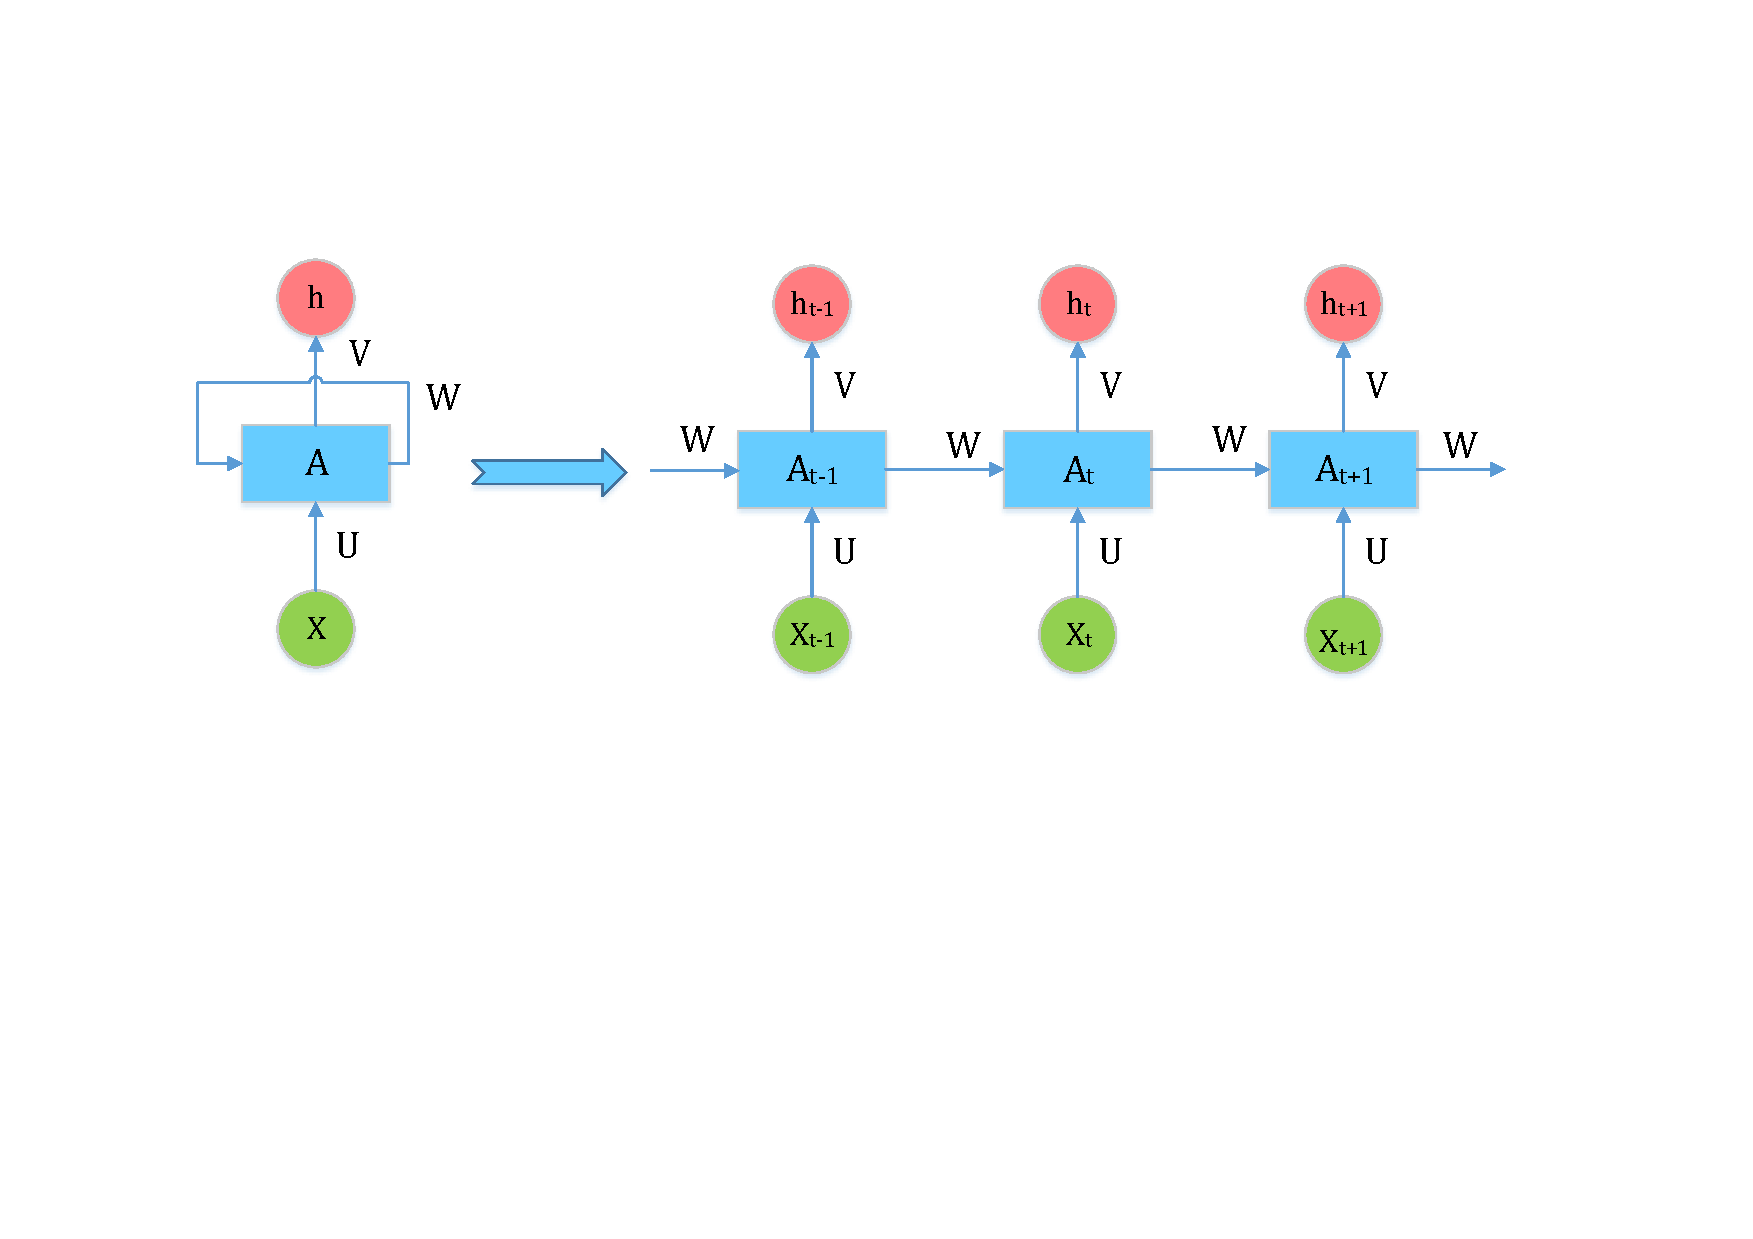
\includegraphics[scale=0.6]{figure/rnn.pdf}
\caption{Architecture of Recurrent Neural Network.}
\label{fig:rnn}
\end{figure}

In a traditional neural network, it is assumed that every input is independent of each other. While, in reality, sometimes, the processed information is in sequence. For example, in a sentence, the words may have relationship with other words. Much as Convolutional Neural Network is especially for data with grid of values, the Recurrent Neural Network is designed to make use of sequential information. The ``recurrent" refers to performing the same task for every element of a sequence, and the input of every node depends on previous computation.

The model of a classical RNN is shown in Figure~\ref{fig:rnn}. In the left of the graph, there is a computation node $\textbf{A}$, with an input $\textbf{X}$, an output for current node $\textbf{h}$. There is a weight $\textbf{W}$ which is utilized to compute next state. In this case, the computation of current state depends on previous computation results. The right side of the figure is the unfolding in time of the computation. From the figure, we can observe that
$$\textbf{A}_t = f(U\textbf{X}_t + W\textbf{A}_{t-1})$$
where $\textbf{A}_t$ is the hidden state of time $\textbf{t}$, $\textbf{X}_t$ is the input of current state, and function $\textbf{f}$ is the transition function for every time step. 
